\documentclass[12pt,compress,aspectratio=169]{beamer}

\mode<presentation>
{
  \usetheme{Singapore}
  \setbeamersize{text margin left=.5cm,text margin right=.5cm}
%  \setbeamertemplate{navigation symbols}{} % suppress nav bar
%  \setbeamercovered{transparent}
}
\usefonttheme{professionalfonts}
\usepackage{amsmath,bm}
\usepackage{siunitx}
\usepackage{tikz}
\usepackage{mathpazo}
\usepackage[scaled]{helvet}
\usepackage{xcolor,colortbl}

\sisetup{
  number-math-rm=\mathnormal,
  per-mode=symbol
}

\usetikzlibrary{decorations.pathmorphing,patterns}


\title{Topic 3: Work and Energy}
\subtitle{Advanced Placement Physics}
\author[TML]{Dr.\ Timothy Leung}
\institute{Olympiads School}
\date{Novemver 16, 2019}

\newcommand{\pic}[2]{\includegraphics[width=#1\textwidth]{#2}}
\newcommand{\mb}[1]{\ensuremath\mathbf{#1}}
\newcommand{\eq}[2]{\vspace{#1}{\Large\begin{displaymath}#2\end{displaymath}}}

\begin{document}

\begin{frame}
  \maketitle
\end{frame}

\begin{frame}
  \frametitle{Files for You to Download}
  \begin{itemize}
  \item Slides for this week and next
    \begin{itemize}
    \item\texttt{PhysAP-03-workEnergy.pdf}--This week's slides on work and
      energy
    \item\texttt{PhysAP-03-momentumImpulse.pdf}--Next week's slides on momentum,
      impulse and general collisions.
    \end{itemize}
  \item\texttt{PhysAP-04-Homework.pdf}--Homework problems for Topics 3 and 4.
  \end{itemize}
  Please download/print the PDF file for the class slides before each class.
  There is no point copying notes that are already printed out for you.
  Instead, take notes on things I say that aren't necessarily on the slides.
  If you want to print the slides, we recommend that you print 4 slides per
  page to save paper.
\end{frame}



\begin{frame}{Work and Energy}
  We start with some definition at are (unfortunately) not very useful:
  \begin{itemize}
    \item \textbf{Energy} is the ability to do work.
    \item \textbf{Work} is the mechanism in which energy is transformed.
  \end{itemize}
  Luckily, we can also use equations to define these concepts.
\end{frame}


\begin{frame}{Work}
  \textbf{Mechanical work} is performed when a force $\mb{F}$ is used to
  displace an object by an infinitesimal amount $d\mb{r}$:

  \eq{-.2in}{
    \boxed{W=\int_{r_1}^{r_2}\mb{F}(r)\cdot d\mb{r}}
  }

  \begin{itemize}
  \item No work done if the force is perpendicular to displacement
    (i.e.\ $\mb{F}\cdot d\mb{r}=0$)
  \item No work done if no displacement ($d\mb{r}=\mb{0}$)
  \item Work can be positive or negative depending on the dot product
    %work done is possible if $\mb{F}$ is opposite direction to
    %$\mb{r}$ ($\mb{F}\cdot d\mb{r}=0$
  \item When there are multiple forces acting on an object, we can compute the
    work done by each \emph{each} force
  \end{itemize}
\end{frame}



\begin{frame}{Kinetic Energy}
  When we apply a force on an object to accelerate it, the resulting amount of
  work done is given by:

  \eq{-.2in}{
    W_{\textrm{net}}=\int\mb{F}_{\textrm{net}}\cdot d\mb{x}=\int m\mb{a}\cdot d\mb{x}
    =m\int\frac{d\mb{v}}{dt}\cdot d\mb{x}
%        
%      \end{align*}
  }

  Since both $\mb{v}$ and $\mb{x}$ are continuous functions in time, we can
  switch the order of differentitation, i.e.:

  \eq{-.2in}{
    =m\int\frac{d\mb{x}}{dt}d\cdot\mb{v}=m\int\mb{v}\cdot d\mb{v}
    =\int_{v_1}^{v_2} mvdv %=\Delta\left(\frac{1}{2}mv^2\right)=\Delta K
  }

  Since $\mb{v}$ and $d\mb{v}$ must be in the same direction, the dot product
  is trivial: $\mb{v}\cdot d\mb{v}=vdv$
\end{frame}



\begin{frame}{Kinetic Energy}
  Continuing from the last slide, this integral, when integrated from
  $v_1$ (initial velocity) to $v_2$ (final velocity):

  \eq{-.2in}{
    m\int_{v_1}^{v_2} vdv=\frac{1}{2}mv^2\Big|^{v_2}_{v_1}=\Delta K
  }
  
  where $\displaystyle K=\frac{1}{2}mv^2$ is defined as the
  \textbf{translational kinetic energy}
\end{frame}



\begin{frame}{Work and Kinetic Energy}
  In fact, the \emph{definition} of kinetic energy came from this integration,
  in that we want to say that work equals to the change in \emph{something},
  and we called that kinetic energy. This is the \textbf{work-energy theorem}:

  \eq{-.15in}{
    \boxed{W_\mathrm{net}=\Delta K}
  }
  \begin{itemize}
  \item\vspace{-.15in} $\Delta K$ can be positive or negative depending on the
    dot product
  \item There may be multiple forces acting on an object; each of the forces
    can add or take away kinetic energy from an object
  \item Therefore we use the ``net'' amount of work done in the above equation
  \end{itemize}
\end{frame}



\begin{frame}{Definition of Work}
  \begin{itemize}
  \item\textbf{Work done by a force}
    \begin{itemize}
    \item We can quantify work by calculating the work done by a specific force
    \item Example: A boy pushes a cart forward. The ``work done by the boy'' is
      the work done by the applied force.
    \end{itemize}
  \item\textbf{Work done on an object}
    \begin{itemize}
    \item There may be more than one force acting on an object
    \item The \emph{sum} of all the work done on the object by each force
    \item The work done by the net force
    \item Also called the \textbf{net work} $W_\mathrm{net}$
    \end{itemize}
  \end{itemize}
\end{frame}



\begin{frame}{Example}
  \textbf{Example 1:} A force $\mb{F}=4.0x\bm{\hat{\imath}}$ (in newtons) acts
  on an object of mass \SI{2.}{\kilo\gram} as it moves from $x=0$ to
  $x=\SI{5.}{\metre}$. Given that the object is at rest at $x=0$,
  \begin{enumerate}[(a)]
  \item Calculate the net work
  \item What is the final speed of the object?
  \end{enumerate}
\end{frame}


\begin{frame}
  \frametitle{Gravitational Force \& Potential Energy}
  The gravitational force (weight) of an object is defined as:
  
  \eq{-.25in}{
    \boxed{\mb{F}_g=m\mb{g}}
  }
  
  For objects near the surface of Earth, we assume that
  $\mb{g}=-g\bm{\hat{\jmath}}=-10\bm{\hat{\jmath}}$
  (in \si{\metre\per\second^2}) is a constant. The work done to raise an object
  from height $h_1$ to $h_2$ is therefore:

  \eq{-.3in}{
    W=\int \mb{F}_g\cdot d\mb{h}
    =\int_{h_1}^{h_2} -mg\bm{\hat{\jmath}}\cdot dh\hat{\bm{\jmath}}
    =-mgh\Big|^{h_2}_{h_1}=-\Delta U_g
  }

  where $U_g=mgh$ is the \textbf{gravitational potential energy}
\end{frame}



%\begin{frame}{Work and Kinetic Energy}
%  Like kinetic energy, the definition of gravitational potential energy came
%  from this integration, in that work equals to the change in \emph{something},
%  and we called that gravitational potential energy.
%
%  \eq{-.2in}{
%    \boxed{W_\mathrm{net}=\Delta U_g}
%  }
%  \begin{itemize}
%  \item\vspace{-.15in} $\Delta U_g$ can be positive or negative depending on
%    the direction of the force
%  \item There may be multiple forces acting on an object; each of the forces
%    can add or take away gravitational potential energy from an object
%  \end{itemize}
%\end{frame}



\begin{frame}
  \frametitle{Spring Force \& Elastic Potential Energy}
  The spring force $\mb{F}_e$ is the force a compressed or stretched spring
  exerts onto objects connected to it. It obeys Hooke's law:
    
  \eq{-.2in}{
    \boxed{\mb{F}_e=-k\mb{x}}
  }

  When applied to the work equation, we can find the work done to
  compress/stretch a spring:

  \eq{-.3in}{
    W=\int\mb{F}_e\cdot d\mb{x}=-k\int xdx=-\frac{1}{2}kx^2\Big|^{x_2}_{x_1}
    =-\Delta U_e
  }
  
  where $U_e=\frac{1}{2}kx^2$ is the \textbf{elastic potential energy}
\end{frame}


\begin{frame}{Conservative Forces}
  Gravitational force, spring force,  electrostatic force (later in the
  course) are called \textbf{conservative forces}
  \begin{itemize}
  \item The work done by these forces relate to a change of another quantity
    called \emph{potential energy}
  \item Since the potential energy is evaluated at the end points, the work
    done by a conservative force is \emph{path independent}
%  \item This force is related to the potential energy by the gradient operator:
%    
%    \eq{-.2in}{
%      \boxed{\mb{F}=-\nabla U=
%        -\frac{\partial U}{\partial x}\bm{\hat{\imath}}
%        -\frac{\partial U}{\partial y}\bm{\hat{\jmath}}
%        -\frac{\partial U}{\partial z}\hat{\bm{k}}
%      }
%    }
%  \item The direction of the force decreases the potential energy and increases
%    the kinetic energy
  \end{itemize}
\end{frame}



\begin{frame}{Conservative Forces}
%  \begin{itemize}
%  \item Gravitational force, spring force,  electrostatic force (later in the
%    course) are called \textbf{conservative forces}
%  \item Work done by a conservative force is independent of the path taken
  Since the expressions for potential energies are obtained by integrating the
  work done by the conservative forces, these forces are therefore the
  negative gradient of the potential energies:

  \eq{-.2in}{
    \boxed{\mb{F}=-\nabla U=
      -\frac{\partial U}{\partial x}\bm{\hat{\imath}}
      -\frac{\partial U}{\partial y}\bm{\hat{\jmath}}
      -\frac{\partial U}{\partial z}\hat{\bm{k}}
    }
  }

  The direction of a conservative force \emph{always} decreases the potential
  energy
\end{frame}




\begin{frame}{Work and Potential Energy}
  Like kinetic energy, the expressions for potential energies come from
  integrating the work equation, in that work equals to the change in
  \emph{something}, and we called that potential energy.

  \eq{-.2in}{
    \boxed{W_\mathrm{net}=-\Delta U}
  }

  $\Delta U$ can be positive or negative depending on the direction of the
  (conservative) force
\end{frame}



\begin{frame}{Conservation of Mechanical Energy}
  Positive work done by conservative forces on an object does two things:
  \begin{enumerate}[1.]
  \item Decrease its potential energy, while
  \item Increase its kinetic energy by the same amount
  \end{enumerate}
  Mathematically, this shows that mechanical energy must always be conserved
  when there are only conservative forces:

  \eq{-.15in}{
    W=-\Delta U = \Delta K \quad\longrightarrow\quad
    \boxed{\Delta K + \Delta U =0}
  }

  That's why those forces are called conservative forces!
\end{frame}



%\begin{frame}
%  \frametitle{The Work-Energy Theorem and Conservation of Energy}
%  Work is equal to the sum of the changing potential and kinetic energy.
%  $K$ is the kinetic energy of objects, and $U$ are all the potential energies.
%
%  \eq{-.2in}{\boxed{W = \Delta U+\Delta K}}
%
%  For an \emph{isolated system}, the net amount of work done to the system
%  by its surrounding must be zero, i.e.\ $W=0$, therefore energy in the system
%  must be conserved
%  
%  \eq{-.2in}{\boxed{U + K = U' + K'}}
%\end{frame}
%
%




\begin{frame}
  \frametitle{Isolated Systems and the Conservation of Energy}
  \begin{itemize}
  \item\textbf{Isolated system:} a system of objects that does not interact with
    the surrounding
  \item ``Interaction'' can be in the form of
    \begin{itemize}
    \item Friction
    \item Exchange of heat
    \item Sound emission
    \end{itemize}
  \item Think of an isolated system as a bunch of objects inside an insulated
    box
  \end{itemize}
  \begin{center}
    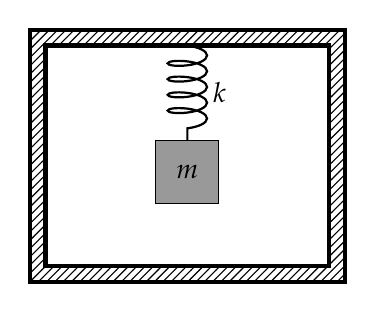
\begin{tikzpicture}[scale=.8]
      \fill[pattern=north east lines] (0,0) rectangle(5,4);
      \draw[ultra thick] (0,0) rectangle(5,4);
      \draw[ultra thick,fill=white](.25,.25) rectangle(4.75,3.75);
      \draw[thick,
        decoration={aspect=.3,segment length=2mm, amplitude=2.5mm, coil},
        decorate] (2.5,3.75)--(2.5,2.25) node[midway,right]{$\;\;k$};
      \draw[fill=black!40](2,2.25) rectangle(3,1.25) node[midway]{$m$};
    \end{tikzpicture}
  \end{center}
\end{frame}


\begin{frame}
  \frametitle{Isolated Systems and Conservation of Energy}
  \begin{itemize}
  \item Since the system is isolated from the surrounding environment, the
    environment can't do any work on it, by definition!
  \item Likewise, the energy inside the system cannot escape either
  \item Therefore energy of the system is conserved
  \item There are \emph{internal} force inside the system that is doing work,
    but the work only converts kinetic energy into potential energies, and vice
    versa.
  \end{itemize}
\end{frame}

\begin{frame}
  \frametitle{Example: Mass sliding on a spring}

  \begin{itemize}
  \item Assuming that there is no friction in any part of the system
  \item The isolated system consists of the mass and the spring 
  \item Energies:
    \begin{itemize}
    \item Kinetic energy of the mass
    \item Elastic potential energy stored in the spring
    \end{itemize}
  \end{itemize}
  \begin{center}
    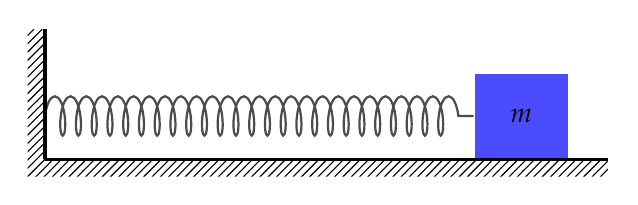
\begin{tikzpicture}[scale=1.1]
      \node[fill=blue!70,inner sep=4.5mm] (a) at (5.5,1) {$m$};
      \draw[thick,draw=black!70,
        decoration={aspect=.3,segment length=2mm, amplitude=2.5mm, coil},
        decorate] (0,1)--(4.95,1);
      \fill [pattern=north east lines] (6.5,.5)--(6.5,.3)--(-.2,.3)
      --(-.2,2)--(0,2)--(0,.5)--cycle;
      \draw[very thick] (0,.5)--(6.5,.5);
      \draw[very thick] (0,.5)--(0,2);
    \end{tikzpicture}
  \end{center}
\end{frame}


\begin{frame}
  \frametitle{Example: Gravity}

  \begin{center}
    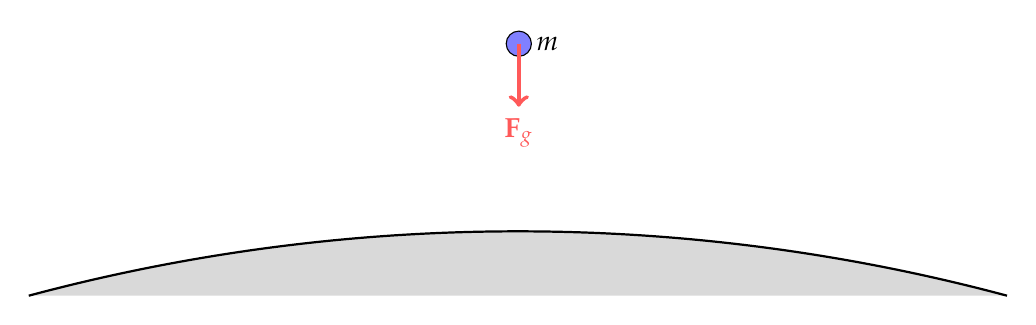
\begin{tikzpicture}[scale=.8]
      \draw[thick,fill=gray!30] (7.75,0) arc(75:105:30);
      \draw[fill=blue!50] (0,4) circle(.2) node[right]{$\;m$};
      \draw[ultra thick, red!65,->] (0,4)--(0,3) node[pos=1,below]{$\mb{F}_g$};
    \end{tikzpicture}
  \end{center}
  
  \begin{itemize}
  \item The isolated system consists of the mass and Earth
  \item Assuming no friction
  \item Energies:
    \begin{itemize}
    \item Kinetic energy of the mass
    \item Gravitational potential energy of the mass
    \end{itemize}
  \end{itemize}
\end{frame}


\begin{frame}
  \frametitle{Example: Vertical spring-mass system}

  \begin{columns}
    \column{.17\textwidth}
    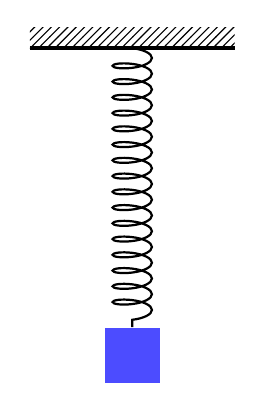
\begin{tikzpicture}[scale=1.3]
      \node[fill=blue!70,inner sep=3.5mm] (b) at (1,2) {};
      \draw[thick,
        decoration={aspect=.3,segment length=2mm, amplitude=2.5mm, coil},
        decorate] (1,5)--(b); 
      \fill [pattern=north east lines] (0,5) rectangle (2,5.2);
      \draw[ultra thick] (0,5)--(2,5);
    \end{tikzpicture}
    \column{.85\textwidth}
    \begin{itemize}
    \item The system consists of a mass, a spring and Earth
    \item Energies:
      \begin{itemize}
      \item Kinetic energy of the mass
      \item Gravitational potential energy of the mass
      \item Elastic potential energy stored in the spring
      \end{itemize}
    \item The total energy of the system is conserved if there is no friction
    \end{itemize}
  \end{columns}
\end{frame}


\begin{frame}
  \frametitle{What if there is friction?}
  Energy is always conserved as long as your system is defined properly

  \begin{columns}
    \column{.2\textwidth}
    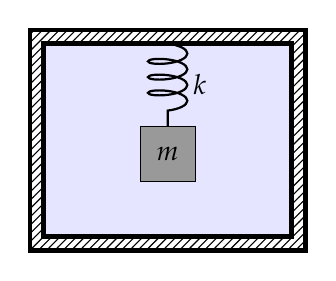
\begin{tikzpicture}[scale=.7]
      \fill[pattern=north east lines] (0,0) rectangle(5,4);
      \draw[ultra thick] (0,0) rectangle(5,4);
      \draw[ultra thick,fill=blue!10](.25,.25) rectangle(4.75,3.75);
      \draw[thick,
        decoration={aspect=.3,segment length=2mm, amplitude=2.5mm, coil},
        decorate] (2.5,3.75)--(2.5,2.25) node[midway,right]{$\;\;k$};
      \draw[fill=black!40](2,2.25) rectangle(3,1.25) node[midway]{$m$};
    \end{tikzpicture}
    \column{.8\textwidth}
    \begin{itemize}
    \item The system consists of a mass, a spring, Earth and all the air
      particles inside the box
    \item As the mass vibrates, friction with air slows it down
    \item While the mass loses energy, the temperature of the air rises due to
      friction
    \item Energies:
      \begin{itemize}
      \item Kinetic and gravitational potential energies of the mass
      \item Elastic potential energy stored in the spring
      \item Kinetic energy of the vibration of the air molecules
      \end{itemize}
    \item Total energy is conserved even as the mass stops moving
    \end{itemize}
  \end{columns}
\end{frame}


\begin{frame}{Conservation of Energy}
  If there are only conservative forces, mechanical energy (i.e.\ $K+U$) is
  always conserved:

  \eq{-.2in}{
    \boxed{K +U =K'+U'}
  }
  
  When there are non-conservative forces, instead of \emph{trying} to isolate
  the system, we can calculate the work done by them $W_{\textrm{nc}}$ and
  add it to the total energy of the system
    
  \eq{-.2in}{
    \boxed{K+U+W_{\textrm{nc}}=K'+U'}
  }
  
  %Work done by $W_{\textrm{nc}}$ are usually friction forces,
  %
\end{frame}



\begin{frame}{Work By Non-Conservative Force}
  Examples of non-conservative forces include:
  \begin{itemize}
  \item Kinetic friction
    \begin{itemize}
    \item $W$ is usually negative
    \item Converts mechanical energy in the system into sound and heat
    \end{itemize}
  \item Applied force
    \begin{itemize}
    \item $W$ may be positive or negative, depending on the problem
    \end{itemize}
  \end{itemize}
  Note that the work-kinetic energy theorem still applies when non-conservative
  forces are present
\end{frame}


\begin{frame}
  \frametitle{Example}
  \textbf{Example 2:} A mass $m$ is dropped from a height of $h$ above the
  equilibrium position of a spring. Set up the equation that determines the
  spring's compression $d$ when the object is instantaneously at rest.
  \begin{center}
    \pic{.35}{spring-example1.png}
  \end{center}
\end{frame}


%\begin{frame}
%  \frametitle{Example}
%  \textbf{Example 3:} A mass $m$ is pulled a distance $d$ up an incline (angle
%  of elevation $\theta$) at constant speed using a rope that is parallel to
%  the incline. The coefficient of friction is $\mu_k$.
%  \begin{enumerate}[(a)]
%  \item What is the magnitude of the tension force in the rope?
%  \item What is the magnitude of the normal force?
%  \item What is the work done by the normal force?
%  \item What is the work done by friction?
%  \item What is the work done by the tension force?
%  \item What is the net work?
%  \item What is the change in total mechanical energy?
%  \item Show that $\Delta E_\mathrm{mech}=W_\mathrm{non-conservative}$.
%  \end{enumerate}
%\end{frame}


\begin{frame}
  \frametitle{Energy Diagrams}
  \begin{itemize}
  \item Plots of potential energy ($U$) vs.\ position for a conservative force
    \begin{center}
      \pic{.5}{energy-diagram.png}
    \end{center}
  \item If more than one conservative force, they can be combined into one graph
  \item Where slope is zero means no force acting on it: it is in a state of
    \textbf{equilibrium}
  \item An object placed at an equilibrium point with $K=0$ will remain there
  \end{itemize}
\end{frame}

%\section{Momentum}
%
%
%\begin{frame}
%  \frametitle{Linear Momentum}
%  \textbf{Linear momentum} is proportional to the object's \textbf{mass} and
%  its \textbf{velocity}.
%
%  \eq{-.2in}{
%    \boxed{\mb{p}=m\mb{v}}
%  }
%  \begin{center}
%    \begin{tabular}{l|c|l}
%      \rowcolor{pink}
%      \textbf{Quantity} & \textbf{Symbol} & \textbf{SI Unit} \\ \hline
%      Momentum & $\mb{p}$ & \si{\kilo\gram.m/s} (kilogram meters per second) \\
%      Mass      & $m$    & \si{\kilo\gram} (kilograms) \\
%      Velocity  & $\mb{v}$ & \si{\metre\per\second} (meters per second) \\
%    \end{tabular}
%  \end{center}
%  \begin{itemize}
%  \item Momentum $\mb{p}$ is a vector in the same direction as velocity
%  \item Like all vectors, $\mb{p}$ obeys \emph{superposition}
%  \end{itemize}
%\end{frame}
%
%\begin{frame}
%  \frametitle{Newton's Second Law of Motion}
%
%  Start with our ``standard form'' of Newton's second law of motion with
%  constant $m$, we can find out how $\Delta\mb{p}$ relates to $\mb{F}$:
% 
%  \eq{-.25in}{
%    \sum\mb{F}=m\mb{a}=m\frac{d\mb{v}}{dt}=\frac{d(m\mb{v})}{dt}
%    =\frac{d\mb{p}}{dt}
%  }
%  \begin{itemize}
%  \item $\mb{F}_\mathrm{net}=\dot{\mb{p}}(t)$ is the general form,
%    $\mb{F}_\mathrm{net}=m\mb{a}$ is a special case
%  \item Momentum is conserved (i.e.\ $\sum\mb{p}$ constant) when the net force
%    on an object or a system of objects is zero.
%  \item Internal forces do not contribute to net force, in that case:
%
%    \eq{-.2in}{
%      \sum_i\mb{p}_i(t_1)=\sum_i\mb{p}_i(t_2)
%    }
%  \end{itemize}
%\end{frame}
%
%\begin{frame}
%  \frametitle{Impulse}
%  Let's get this by looking at Newton's 2nd law again. If we rearrange the
%  variables:
%  
%  \eq{-.2in}{
%    \mb{F}_\mathrm{net}=\frac{d\mb{p}}{dt}\;\rightarrow\;
%    \mb{F}_\mathrm{net}dt=d\mb{p}
%  }
%  We can integrate both sides to get the \textbf{impulse-momentum theorem}.
% 
%  \eq{-.2in}{
%    \boxed{
%      \mb{J}_\mathrm{net}
%      =\int_{t_1}^{t_2}\mb{F}_\mathrm{net}dt
%      =\int d\mb{p}=\Delta\mb{p}}
%  }
%  The quantity $\mb{J}$ is called the impulse.
%\end{frame}
%
%
%\begin{frame}
%  \frametitle{Impulse}
%  \begin{itemize}
%  \item $\mb{F}$, $\mb{p}$ and $\mb{J}$ are all vectors, so the integral can
%    be evaluated in each of the $x$, $y$ and $z$ axis, i.e., for the $x$
%    direction:
%
%    \eq{-.25in}{
%      J_x=\int_{t_1}^{t_2}F_xdt=\int dp_x=\Delta p_x
%    }
%
%  \item\textbf{Average force:} is a ``force'' that gets the same impulse, i.e.
%
%    \eq{-.2in}{
%      \overline{\mb{F}}=\frac{\int_{t_1}^{t_2}\mb{F}dt}{t_2-t_1}
%      =\frac{\mb{J}}{\Delta t}
%     }
%  \item Note that impulse from each individual force does not depend on whether
%    the object moves
%  \end{itemize}
%\end{frame}
%
%\begin{frame}
%  \frametitle{Impulse: An Example}
%  \textbf{Example 4:} Jim pushes a box with mass \SI{1.}{\kilo\gram} with a
%  \SI{5.}{\newton} force for \SI{10}{\second} while the box stays on the same
%  place. Find the impulse of the pushing force, friction force, the
%  gravitational force, and the net force.
%\end{frame}
%
%\begin{frame}
%  \frametitle{Impulse: Another Example}
%  \textbf{Example 5:} Two balls of the same mass are dropped from the same
%  height onto the floor. The first ball bounces upwards from the floor
%  elastically. The second ball sticks to the floor. The first applies an
%  impulse to the floor of $I_1$ and the second applies an impulse $I_2$. The
%  two impulses obey:
%  \begin{enumerate}[(a)]
%  \item $I_2=2I_1$
%  \item $I_2=I_1/2$
%  \item $I_2=4I_1$
%  \item $I_2=I_1/4$
%  \end{enumerate}
%\end{frame}
%
%\begin{frame}
%  \frametitle{Conservation of Momentum}
%  \begin{itemize}
%  \item From Newton's third law, we know that the action and reaction forces are
%    always equal in magnitude and in opposite direction. Thus, their total
%    impulse would be zero. 
%    
%  \item When there is no external force, the momentum of the total system will
%    always be constant. We saw that a few slides ago:
%
%    \eq{-.2in}{
%      \sum\mb{p}(t_1)=\sum\mb{p}(t_2)
%    }
%  \end{itemize}
%\end{frame}
%
%\begin{frame}
%  \frametitle{How to Solve Conservation of Momentum Problem}
%  \begin{enumerate}
%  \item Check whether the condition for the conservation of momentum is
%    satisfied.
%  \item If so, write out expressions for initial momentum and final momentum,
%    and equate the two. You will get $1$ to $3$ equations (one for each
%    direction).
%  \item Solve these equations, find the quantity you need to find.
%  \end{enumerate}
%%\end{frame}
%%
%%\begin{frame}
%%  \frametitle{Two Remarks}
%%  \begin{itemize}
%%  \item Sometimes, the external force \emph{does} exist, but are too small, or
%%    the time interval of the external force is very short. In these cases, we
%%    can still regard the total momentum as conserved.
%  Remember that momentum is a vector. If there is no external force component
%  in some direction, then the momentum component in this direction is still
%  conserved.
%%  \end{itemize}
%\end{frame}
%
%\begin{frame}
%  \frametitle{Example}
%  \textbf{Example 6:} Two blocks A and B, both have mass \SI{1.}{\kilo\gram}.
%  Block A has velocity \SI{3.}{\metre\per\second} and block B is at rest. Their
%  distance is \SI{1.}{\metre}. The surface is has dynamic friction coefficient
%  $0.02$. After they collide, they move together, what would be the final
%  velocity of these two blocks? How far can they go after the collision?
%\end{frame}
%
%%\begin{frame}
%%  \frametitle{More Example}
%%  Max throws a ball into the air with an initial speed $\SI{10}{\metre\per\second} at an
%%  angle of $60$ degree with the horizontal direction. By accident, the ball
%%  splits into two parts (horizontally) in the air. Suppose both parts land at
%%  the same time, neglecting the air resistance,
%%  \begin{enumerate}
%%  \item If one part is \SI{5}{\m} away from its original position (same
%%    direction as the initial speed), where is the second part?
%%  \item How about one parties \SI{5}{\metre} away from the original position in the
%%    direction that has an angle of $30$ degree with its initial speed?
%%  \end{enumerate}
%%\end{frame}
%%
%\begin{frame}
%  \frametitle{Before We Dive Into Some Exercises}
%  \begin{itemize}
%  \item The most typical applications of momentum conservation are collision
%    and explosions
%  \item\textbf{Collision: object A hits object B}. Regardless of whether they
%    move together or not afterwards, momentum is conserved.
%    \begin{itemize}
%    \item Head-on collisions are usually 1D
%    \item Glancing collisions are usually 2D or 3D.
%    \end{itemize}
%  \item\textbf{Explosion: A explodes and becomes B and C (and D and E\ldots)}.
%    Total momentum of B and C (and D and E\ldots) is the same as A in the
%    beginning. 
%  \end{itemize}
%\end{frame}
%
%\begin{frame}
%  \frametitle{Collision Problem}
%  \textbf{Example 7:} Two objects with equal mass are heading toward each
%  other with equal speeds, undergo a head-on collision. Which one of the
%  following statement is correct?
%  \begin{enumerate}[(a)]
%  \item Their final velocities are zero
%  \item Their final velocities may be zero
%  \item Each must have a final velocity equal to the other's initial velocity
%  \item Their velocities must be reduced in magnitude
%  \end{enumerate}
%\end{frame}
%
%\begin{frame}
%  \frametitle{Conservation of Momentum Example}
%  \textbf{Example 8:} Two astronauts, each of mass \SI{75}{\kilo\gram}, are
%  floating next to each other in space, outside the space shuttle. One of them
%  pushes the other through a distance of \SI{1.}{\metre} (about an arm's
%  length) with a force of \SI{300}{\newton}. What is the final relative
%  velocity of the two?
%  \begin{enumerate}[(a)]
%  \item \SI{2.}{\metre\per\second}
%  \item \SI{2.83}{\metre\per\second}
%  \item \SI{4.}{\metre\per\second}
%  \item \SI{16.}{\metre\per\second}
%  \end{enumerate}
%\end{frame}
%
%\begin{frame}
%  \frametitle{Continuous Problems in the Application of Momentum}
%
%%  \textbf{Example 9:} A water fountain sprays water with a flow of
%%  \SI{30}{L/min}. Suppose the water has no initial velocity, find the impulse
%%  of the pushing force in $1$ hour and estimate the pushing force, assuming the
%%  force is constant.
%%\end{frame}
%%
%%\begin{frame}
%%  \frametitle{Example: Rocket Thrust}
%  \textbf{Example 10:} A rocket generates a thrust force by ejecting hot gases
%  from an engine. If it takes \SI{1}{\milli\second} to combust
%  \SI{1.}{\kilo\gram} of fuel, ejecting it at a speed of
%  \SI{1000}{\metre\per\second}, what thrust is generated?
%  \begin{enumerate}[(a)]
%  \item \SI{1000}{\newton}
%  \item \SI{10000}{\newton}
%  \item \SI{100000}{\newton}
%  \item \SI{1000000}{\newton}
%  \end{enumerate}
%\end{frame}
%
%\begin{frame}
%  \frametitle{Another Space Example}
%  \textbf{Example 11:} A rocket for mining the asteroid belt is designed like a
%  large scoop. It is approaching asteroids at a velocity of
%  \SI{e4}{\metre\per\second}. The asteroids are much smaller than the rocket.
%  If the rocket scoops asteroids at a rate of \SI{100}{\kilo\gram\per\second},
%  what thrust (force) must the rocket's engine provide in order for the rocket
%  to maintain constant velocity? Ignore any variation in the rocket's mass due
%  to the burning fuel.
%  \begin{enumerate}[(a)]
%  \item \SI{e3}{\newton}
%  \item \SI{e6}{\newton}
%  \item \SI{e9}{\newton}
%  \item \SI{e12}{\newton}
%  \end{enumerate}
%\end{frame}
%
%
%\begin{frame}
%  \frametitle{Example}
%  \textbf{Example 12:} A ball is dropped from a height $h$. It hits the ground
%  and bounces up with a momentum loss of $10\%$ due to the impact. The maximum
%  height it will reach is:
%  \begin{enumerate}[(a)]
%  \item $0.90h$
%  \item $0.81h$
%  \item $0.949h$
%  \item $0.3h$
%  \end{enumerate}
%\end{frame}
%
%\begin{frame}
%  \frametitle{Conservation of Energy Example}
%  \textbf{Example 13:} A simple pendulum has a bob of mass \SI{2}{\kilo\gram}
%  hanging on a cord of length \SI{1}{\metre}. Suppose the pendulum is raised
%  until it is horizontal (and angular displacement of \ang{90}) and then
%  released. What is the speed of the bob at the bottom of its swing?
%  \begin{enumerate}[(a)]
%  \item\SI{9.91}{\metre\per\second}
%  \item\SI{19.6}{\metre\per\second}
%  \item\SI{3.13}{\metre\per\second}
%  \item\SI{4.43}{\metre\per\second}
%  \end{enumerate}
%\end{frame}
% 
%\begin{frame}
%  \frametitle{Conservation of Energy Example}
%  \textbf{Example 14:} A toy firing a ball vertically consists of a vertical
%  spring which is compressed by \SI{.10}{\metre}. A force of \SI{10.}{\newton}
%  is needed to hold the spring at that compression. If a ball of mass
%  \SI{.050}{\kilo\gram} is placed on the compressed spring and the spring is
%  released, the ball will reach a height (above its initial position) of:
%  \begin{enumerate}[(a)]
%  \item \SI{1.}{\metre}
%  \item \SI{1.2}{\metre}
%  \item \SI{1.4}{\metre}
%  \item \SI{1.6}{\metre}
%  \end{enumerate}
%\end{frame}
%
%
%\section{Elastic Collisions}
%
%\begin{frame}
%  \frametitle{Classifications of Collisions}
%  \begin{itemize}
%  \item Elastic Collision:
%    \begin{itemize}
%    \item Total kinetic energy is conserved
%    \item<alert@2> Momentum is conserved
%    \end{itemize}
%  \item Inelastic collision:
%    \begin{itemize}
%    \item Kinetic energy is \textbf{not} conserved
%    \item<alert@2> Momentum is conserved
%    \end{itemize}
%  \item Completely inelastic collision:
%    \begin{itemize}
%    \item ``Perfectly inelastic collision''
%    \item The objects move together after the collision
%    \item Kinetic energy is \textbf{not} conserved
%    \item<alert@2> Momentum is conserved
%    \end{itemize}
%  \end{itemize}
%\end{frame}
%
%\begin{frame}
%  \frametitle{Elastic Collision}
%  If two objects 1 and 2 of mass $m_1$ and $m_2$ and initial velocities
%  $v_{1,i}$ and $v_{2,i}$ collide elastically, their final velocities will be:
%  
%  {\Large
%    \begin{displaymath}
%      v_{1,f}=\frac{v_{1,i}(m_1-m_2)+2m_2v_{2,i}}{m_1+m_2}
%    \end{displaymath}
%    
%    \begin{displaymath}
%      v_{2,f}=\frac{v_{2,i}(m_2-m_1)+2m_1v_{1,i}}{m_1+m_2}
%    \end{displaymath}
%  }
%\end{frame}
%
%\begin{frame}
%  \frametitle{Elastic Collision Example}
%
%  \textbf{Example 15:} Blocks A and B have the same mass; A hits B with a speed
%  of \SI{5.}{\metre\per\second} while B is initially at rest. If the collision
%  is elastic, what would be the final speed of these two objects?
%\end{frame}
%
%
%\begin{frame}
%  \frametitle{Elastic Collision Example}
%  \textbf{Example 16:} Blocks A and B with the same mass; A has a velocity
%  \SI{3.}{\metre\per\second} to the east while B has \SI{2}{\metre\per\second}
%  to the west. If the collision is elastic, after the collision, what would the
%  velocity of the two blocks be?
%\end{frame}
%
%
%\begin{frame}
%  \frametitle{Elastic Collision Example}
%  
%  \textbf{Example 17:} Throw a ball to a really big wall, when the ball reaches
%  the wall, it has a velocity \SI{10}{\metre\per\second} toward the wall. If
%  the collision is elastic, what would the final velocity of the ball be?
%\end{frame}
%
%
%\begin{frame}
%  \frametitle{Elastic Collision Example}
%  \textbf{Example 18:} Throw a ball with a velocity \SI{4.}{\metre\per\second}
%  toward a train with a velocity \SI{40}{\metre\per\second} toward the ball.
%  If the collision is elastic, what would the final velocity of the ball be?
%\end{frame}
%
%
%\begin{frame}
%  \frametitle{Inelastic Collision: Calculating Energy Loss}
%  \textbf{Example 19:} Two blocks A and B with mass \SI{2.}{\kilo\gram}, block
%  A hits B with velocity \SI{4.}{\metre\per\second} while B is at rest.
%  \begin{enumerate}[(a)]
%  \item Suppose the collision is completely inelastic, what would the final
%    velocity of A and B be?
%  \item What is the loss of energy?
%  \end{enumerate}
%\end{frame}
%
\end{document}
